%!TeX program = xelatex
\documentclass{SYSUReport}
\usepackage{amsmath}
\usepackage{amssymb}
\usepackage{tikz}
\usepackage{adjustbox}
\usepackage{booktabs}
\usepackage{multirow}
\usepackage{graphicx}
\usepackage{longtable}
\usepackage{listings}
\usepackage{xcolor}
\usepackage{hyperref}

\lstdefinestyle{mystyle}{
    backgroundcolor=\color{gray!10},
    basicstyle=\ttfamily\small,
    keywordstyle=\color{blue!70!black},
    commentstyle=\color{green!40!black},
    stringstyle=\color{purple!60!black},
    numbers=left,
    numberstyle=\tiny\color{gray},
    frame=single,
    breaklines=true,
    captionpos=b
}
\lstset{style=mystyle}

\headl{24347014 陈泳强}
\headr{实验三：百万富翁问题与不经意传输}
\lessonTitle{数据安全和隐私保护}
\reportTitle{实验三：百万富翁问题与不经意传输}
\stuname{陈泳强}
\stuid{24347014}
\inst{网络空间安全学院}
\major{网络空间安全}
\date{2026 年 11 月 11 日}

\begin{document}

\cover
\thispagestyle{empty}
\clearpage

\tableofcontents
\clearpage

\pagenumbering{arabic}
\setcounter{page}{1}

% =========================================================
\section{实验要求与环境}

\subsection{实验要求}

本实验在半诚实模型下本地模拟两方计算与消息交换，分为基础实验与拓展实验两部分，合并提交一份报告。

\textbf{基础实验：百万富翁问题。}Alice 与 Bob 分别持有财富 $a$ 和 $b$，希望仅获知 $a$ 是否严格大于 $b$：成立输出 1，否则输出 0，相等也输出 0。基础输入范围为 $0\sim 255$。要求自行实现两方比较协议，不能调用直接完成整个比较任务的封装接口；程序中分别保存双方财富及各自秘密信息，明确双方交换的消息；完成固定输入与至少 20 对随机输入测试，并检查负数、256 和非整数输入；比较 $0\sim 15$、$0\sim 63$、$0\sim 255$ 三个范围下的运行开销；分析双方收到的消息是否额外暴露对方财富，并讨论多次查询推断问题。

\textbf{拓展实验：不经意传输与隐私查表。}发送方持有两条消息 $m_0,m_1$，接收方持有选择位 $c$，通过 2 选 1 OT 取得所选消息。要求自行实现 OT 协议，不得用普通条件选择代替；分别选择第 0 条和第 1 条消息各测试至少 10 组随机消息；测试两条消息相同、选择位不合法的情况；与“直接发送两条明文”“告知选择后只发所选”两种方法比较；比较 16、64、256 字节消息长度对运行开销的影响；选做 4 选 1 OT。

\textbf{选做完成情况：}本报告完成了两项选做任务——基础部分的“多次查询推断 Alice 财富”分析（第 \ref{sec:query} 节），以及拓展部分的 4 选 1 OT（第 \ref{sec:ot41} 节）。

\subsection{实验环境}

\begin{itemize}
  \item 操作系统：Windows 11，终端 Git Bash（MINGW64）
  \item Python 环境：conda 环境 \texttt{he}，Python 3.12.15
  \item 依赖库：\texttt{sympy} 1.14.0（RSA 素数生成与模逆）；Paillier 复用实验四的独立实现 \texttt{experiment4/paillier/paillier.py}
  \item 报告编译：Overleaf + XeLaTeX，模板 \texttt{SYSUReport.cls}
  \item 代码仓库：\url{https://github.com/Skylarkyq06/research-tools-weeks}，实验三代码位于 \texttt{experiment3/}
\end{itemize}

\subsection{代码与数据目录}

\begin{lstlisting}[language=bash, caption={实验三代码与数据目录}]
experiment3/
|-- common/channel.py            # 模拟消息通道，统计发送字节数
|-- millionaire/
|   |-- paillier_compare.py      # Paillier 安全比较协议 + 输入校验
|   |-- benchmark.py             # 三个范围的耗时/字节数基准
|   `-- query_attack.py          # 多次查询推断分析（选做）
|-- ot/
|   |-- ot_rsa.py                # RSA 盲化 1-out-of-2 与 4-out-of-1
|   `-- ot_benchmark.py          # OT 正确性与长度对比
`-- results/                     # 6 个 CSV，报告所有数字均来源于此
\end{lstlisting}

% =========================================================
\section{基础实验：百万富翁问题}

\subsection{协议选择}

直接比较明文会泄露双方财富，因此需要构造一条“只暴露比较结果、不暴露输入”的交互协议。本实验采用 \textbf{Paillier 同态加密}实现安全比较，核心思路是把 $a>b$ 的判断转化为 $a-b>0$ 的判断，并利用 Paillier 的加法同态性，让 Bob 在不知道 $a$ 的情况下计算 $E(a-b)$，再由 Alice 解密并只公布差值的符号。

Paillier 加密满足：
\begin{equation}
E(m_1)\cdot E(m_2)\bmod n^2 = E(m_1+m_2\bmod n),
\end{equation}
且对负数 $-b$ 可写成 $E(-b\bmod n)$。因此 $E(a)\cdot E(-b)=E(a-b\bmod n)$，整个过程中 Bob 不接触 $a$，Alice 不接触 $b$。

\subsection{双方计算与消息交换过程}

设 Alice 持有 $a$，Bob 持有 $b$，双方约定结果公开（百万富翁问题的标准设定：双方都知道 $a>b$ 是否成立）。

\begin{center}
\begin{tikzpicture}[scale=0.9]
  \node (A) at (0,0) {\textbf{Alice}（持有 $a$）};
  \node (B) at (8,0) {\textbf{Bob}（持有 $b$）};
  \draw[thick] (0.9,0) -- (7.1,0);
  \draw[->,thick] (0.9,0.5) -- node[above] {1. $pk$，$E(a)$} (7.1,0.5);
  \draw[->,thick] (7.1,-0.5) -- node[below] {2. $E(a-b)=E(a)\cdot E(-b)\bmod n^2$} (0.9,-0.5);
  \node at (4,-1.3) {3. Alice 用 $sk$ 解密得到 $(a-b)\bmod n$，判定符号并公布结果};
\end{tikzpicture}
\end{center}

具体步骤：

\begin{enumerate}
  \item Alice 调用 \texttt{keygen(1024)} 生成 Paillier 密钥对 $(pk,sk)$，加密自己的财富得到 $c_a=E(a)$，把 $(pk,c_a)$ 发送给 Bob。这一步 Alice 保存 $a$ 与 $sk$，Bob 收到 $pk$ 与 $c_a$。
  \item Bob 用自己的财富计算 $c_{-b}=E(-b\bmod n)$，利用同态性计算 $c_{diff}=c_a\cdot c_{-b}\bmod n^2=E(a-b\bmod n)$，把 $c_{diff}$ 发回 Alice。Bob 保存 $b$ 与 $c_{diff}$ 的计算中间值，Alice 收到 $c_{diff}$。
  \item Alice 用 $sk$ 解密得到 $d=(a-b)\bmod n$。由于 $a,b\in[0,255]$ 且 $n$ 为 1024 位，$|a-b|<n/2$，所以：
  \begin{itemize}
    \item $d=0$：$a=b$，输出 0；
    \item $0<d\le n/2$：$a>b$，输出 1；
    \item $d>n/2$：实际差值为负，$a<b$，输出 0。
  \end{itemize}
\end{enumerate}

整个协议共 \textbf{2 轮、3 条消息}：Alice$\to$Bob 发 $pk$ 和 $E(a)$，Bob$\to$Alice 发 $E(a-b)$。没有调用任何现成的比较封装接口，同态乘法、解密和符号判定全部手写。

\subsection{输入合法性校验}

程序在协议入口对双方输入做严格校验，拒绝负数、超出当前范围的值、非整数以及布尔值（Python 中 \texttt{bool} 是 \texttt{int} 的子类，必须单独排除）。

\begin{lstlisting}[language=Python, caption={输入校验函数}]
def validate_wealth(value, name="wealth", max_val=255):
    if not isinstance(value, int) or isinstance(value, bool):
        raise TypeError(f"{name} 必须为整数，收到 {type(value).__name__}: {value!r}")
    if value < 0:
        raise ValueError(f"{name} 不能为负数：{value}")
    if value > max_val:
        raise ValueError(f"{name} 超出当前范围（0~{max_val}）：{value}")
    return True
\end{lstlisting}

\subsection{关键代码：同态减法与符号判定}

\begin{lstlisting}[language=Python, caption={Paillier 安全比较核心片段}]
# 1. Alice 生成密钥并加密 a
pub, priv = keygen(key_bits)
n = pub.n
ca = encrypt(pub, a)                       # E(a)

# 2. Bob 计算 E(a-b) = E(a) * E(-b) mod n^2
cb_neg = encrypt(pub, (-b) % n)            # E(-b mod n)
c_diff = (ca * cb_neg) % (n ** 2)          # 同态加法

# 3. Alice 解密并判定符号
diff = decrypt(priv, c_diff)               # (a - b) mod n
if diff == 0:
    result = 0                             # a == b
elif diff <= n // 2:
    result = 1                             # a > b
else:
    result = 0                             # a < b
\end{lstlisting}

\subsection{固定输入测试}

固定用例覆盖相等、严格大于、严格小于和边界值，全部通过：

\begin{table}[h]
\centering
\caption{固定输入测试结果}
\begin{tabular}{cccccc}
\toprule
$a$ & $b$ & 预期输出 & 实际输出 & 是否通过 \\
\midrule
0   & 0   & 0 & 0 & 通过 \\
255 & 255 & 0 & 0 & 通过 \\
128 & 127 & 1 & 1 & 通过 \\
127 & 128 & 0 & 0 & 通过 \\
1   & 1   & 0 & 0 & 通过 \\
42  & 42  & 0 & 0 & 通过 \\
254 & 255 & 0 & 0 & 通过 \\
255 & 254 & 1 & 1 & 通过 \\
0   & 255 & 0 & 0 & 通过 \\
255 & 0   & 1 & 1 & 通过 \\
\bottomrule
\end{tabular}
\end{table}

\subsection{非法输入测试}

\begin{table}[h]
\centering
\caption{非法输入测试结果}
\begin{tabular}{lll}
\toprule
输入 & 异常类型 & 提示信息 \\
\midrule
$-1$      & \texttt{ValueError} & 不能为负数 \\
$256$     & \texttt{ValueError} & 超出当前范围（0$\sim$255） \\
$3.5$     & \texttt{TypeError}  & 必须为整数，收到 float \\
\texttt{'100'} & \texttt{TypeError} & 必须为整数，收到 str \\
\texttt{True}  & \texttt{TypeError} & 必须为整数，收到 bool \\
\bottomrule
\end{tabular}
\end{table}

\subsection{20 对随机输入测试}

在 $[0,255]$ 内随机生成 20 对财富，每对运行一次完整协议（每次重新生成密钥和加密随机数），全部通过：

\begin{longtable}{cccc|cccc}
\caption{20 对随机输入测试结果}\\
\toprule
$a$ & $b$ & 预期 & 实际 & $a$ & $b$ & 预期 & 实际 \\
\midrule
\endfirsthead
\toprule
$a$ & $b$ & 预期 & 实际 & $a$ & $b$ & 预期 & 实际 \\
\midrule
\endhead
227 & 137 & 1 & 通过 & 101 & 41  & 1 & 通过 \\
176 & 80  & 1 & 通过 & 26  & 241 & 0 & 通过 \\
234 & 160 & 1 & 通过 & 161 & 44  & 1 & 通过 \\
56  & 92  & 0 & 通过 & 56  & 185 & 0 & 通过 \\
37  & 21  & 1 & 通过 & 217 & 121 & 1 & 通过 \\
242 & 244 & 0 & 通过 & 128 & 155 & 0 & 通过 \\
128 & 72  & 1 & 通过 & 248 & 239 & 1 & 通过 \\
147 & 185 & 0 & 通过 & 238 & 67  & 1 & 通过 \\
59  & 139 & 0 & 通过 & 103 & 85  & 1 & 通过 \\
100 & 38  & 1 & 通过 & 85  & 212 & 0 & 通过 \\
\bottomrule
\end{longtable}

\begin{figure}[h]
\centering
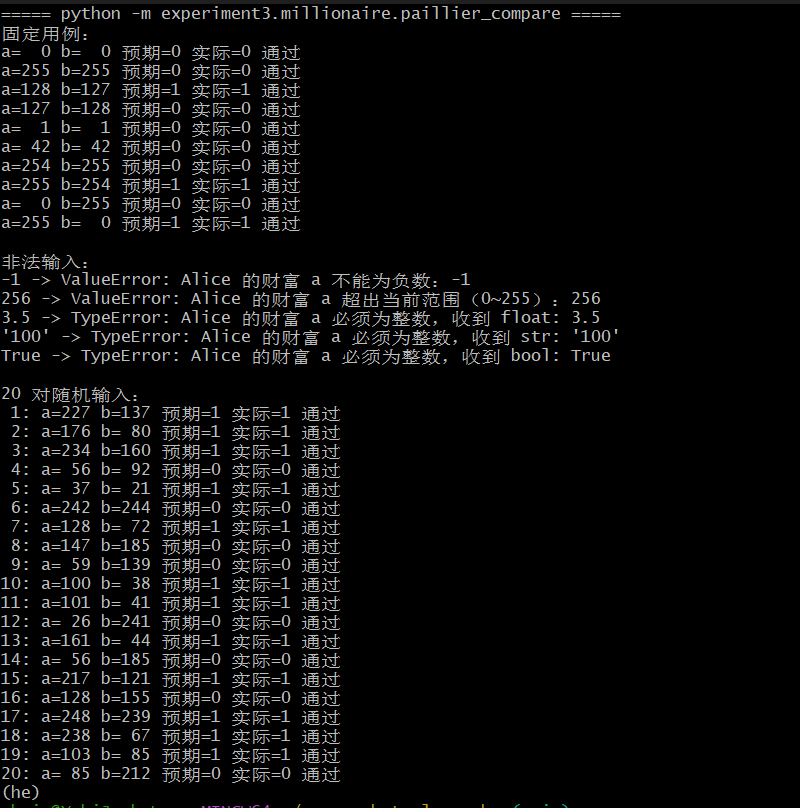
\includegraphics[width=0.92\textwidth]{figures/paillier_test.png}
\caption{Paillier 安全比较测试输出（固定用例、非法输入与 20 对随机用例全部通过）}
\label{fig:paillier-test}
\end{figure}

\subsection{不同取值范围下的运行开销}

在 $0\sim 15$、$0\sim 63$、$0\sim 255$ 三个范围内各随机生成 10 对财富，每对运行 3 次，每次重新生成 Paillier 密钥（1024 位）。密钥生成时间单独记录，协议耗时指总耗时减去密钥生成。结果如下：

\begin{table}[h]
\centering
\caption{三个取值范围下的平均耗时与传输字节数（每组 30 次）}
\begin{tabular}{cccccc}
\toprule
范围 & 次数 & 平均总耗时 (s) & 其中密钥生成 (s) & 协议耗时 (s) & 平均字节数 \\
\midrule
$0\sim 15$  & 30 & 0.1207 & 0.0874 & 0.0333 & 896.0 \\
$0\sim 63$  & 30 & 0.1481 & 0.1148 & 0.0333 & 896.0 \\
$0\sim 255$ & 30 & 0.1247 & 0.0915 & 0.0332 & 896.0 \\
\bottomrule
\end{tabular}
\end{table}

\textbf{分析：}三个范围的\textbf{平均字节数完全相同（896.0 字节）}，\textbf{协议耗时几乎恒定（0.0332--0.0333 s）}。总耗时的波动来自密钥生成（0.087--0.115 s），这是随机素数生成的抖动，与输入范围无关。原因是 Paillier 密文长度由模数 $n$ 的位数决定：1024 位密钥下 $n$ 为 128 字节、$n^2$ 为 256 字节，公钥（$n$ 与 $g$）约 384 字节，两个密文各 256 字节，合计 $384+256+256=896$ 字节。只要明文 $<n$，输入范围扩大不会改变密文长度，也不会改变同态乘法和解密的计算量。因此\textbf{取值范围扩大后，耗时和传输数据量都不变}，开销由安全参数主导，而非输入数值大小。

% =========================================================
\section{基础实验的隐私分析}

\subsection{双方收到的消息是否额外暴露对方财富}

\textbf{Bob 的视角。}Bob 收到 $pk$ 和 $E(a)$。Paillier 是语义安全的：在标准假设下，给定 $E(a)$ 和公钥，Bob 无法区分 $E(a)$ 对应的是 $a$ 还是 $a'$，因此 Bob 无法从密文中得到 $a$ 的任何信息。Bob 自己计算 $E(-b)$ 和 $E(a-b)$，全程没有接触 $a$ 的明文。

\textbf{Alice 的视角。}Alice 解密得到 $d=(a-b)\bmod n$。由于 Alice 知道 $a$，她能推出的关于 $b$ 的信息恰好是：
\begin{itemize}
  \item 若结果为 1（$a>b$），则 $b\in[0,a-1]$；
  \item 若结果为 0 且 $a>b$ 不成立，则 $b\in[a,255]$（相等时 $b=a$）。
\end{itemize}
这正是“已知自己的输入和约定输出”本身可推得的信息，符合半诚实模型的隐私目标——协议没有\textbf{额外}暴露 $b$ 的精确值。例如 $a=254$ 且输出 0 时，Alice 只能推出 $b\in\{254,255\}$，无法区分两者。

\subsection{多次查询推断 Alice 的财富（选做）}
\label{sec:query}

单次协议只输出 1 比特，但当 Bob 可以固定 Alice 的 $a$、反复用不同的 $b$ 发起比较时，返回的 0/1 序列组合起来会泄露更多信息。本实验实现两种查询策略：

\begin{itemize}
  \item \textbf{二分查询}：维护区间 $[lo,hi]$，每次取中点 $mid$，比较 $a>mid$，根据结果收缩区间。查询次数上界为 $\lceil\log_2 256\rceil=8$。
  \item \textbf{线性扫描}：从 $b=0$ 开始逐个询问，找第一个使 $a>b$ 不成立的 $b$，此时 $a=b$。查询次数为 $a+1$，最坏 256 次。
\end{itemize}

为贴近真实场景，所有查询复用同一对 Paillier 密钥（Alice 的密钥在一次会话内固定），只重新生成加密随机数。20 个二分样本全部推断正确，每次恰好 8 次查询；5 个线性样本也全部正确，查询次数分别为 1、2、43、129、256。

\begin{table}[h]
\centering
\caption{二分查询与线性查询的推断结果（节选）}
\begin{tabular}{cccccc}
\toprule
\multirow{2}{*}{$a$} & \multicolumn{2}{c}{二分查询} & \multicolumn{2}{c}{线性查询} \\
\cmidrule(lr){2-3}\cmidrule(lr){4-5}
 & 推断值 & 次数 & 推断值 & 次数 \\
\midrule
0   & 0   & 8 & 0   & 1 \\
1   & 1   & 8 & 1   & 2 \\
42  & 42  & 8 & 42  & 43 \\
128 & 128 & 8 & 128 & 129 \\
255 & 255 & 8 & 255 & 256 \\
\bottomrule
\end{tabular}
\end{table}

二分 20 个样本平均查询 8.00 次，线性 5 个代表样本平均 86.20 次，二分的加速比约 \textbf{10.8 倍}。

\textbf{讨论：}单次协议只泄露 1 比特，单次运行内隐私目标成立；但比较函数本身是一个“黑盒比较器”，多轮查询的\textbf{结果组合}允许 Bob 用二分法在 8 次内定位 $0\sim255$ 内的任意 $a$。这不是协议实现“额外暴露”了 $b$，而是输出函数在多轮查询下的固有可推断性。防御思路包括限制同一对输入的查询次数、对结果加噪（差分隐私）或引入查询预算。

\begin{figure}[h]
\centering
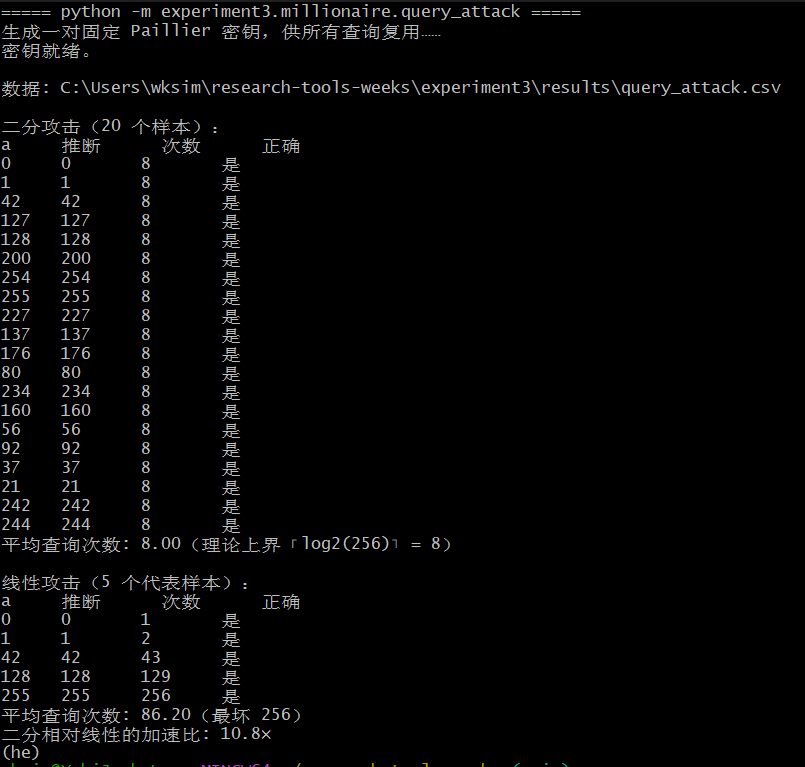
\includegraphics[width=0.85\textwidth]{figures/query_attack.png}
\caption{多次查询推断输出（二分 20 个样本均 8 次定位，线性最坏 256 次）}
\label{fig:query-attack}
\end{figure}

% =========================================================
\section{拓展实验：不经意传输}

\subsection{协议选择与消息流}

采用经典的 \textbf{RSA 盲化 1-out-of-2 OT}。发送方 S 持有 $m_0,m_1$，接收方 R 持有选择位 $c\in\{0,1\}$。协议如下：

\begin{center}
\begin{tikzpicture}[scale=0.85]
  \node (S) at (0,0) {\textbf{发送方 S}（$m_0,m_1$）};
  \node (R) at (9,0) {\textbf{接收方 R}（$c$）};
  \draw[thick] (1.3,0) -- (7.7,0);
  \draw[->,thick] (1.3,0.7) -- node[above] {1. $N,e,x_0,x_1$} (7.7,0.7);
  \draw[->,thick] (7.7,0) -- node[above] {2. $v=(x_c+k^e)\bmod N$} (1.3,0);
  \draw[->,thick] (1.3,-0.7) -- node[below] {3. $M_i=(m_i+k_i)\bmod N,\ i=0,1$} (7.7,-0.7);
  \node at (4.5,-1.5) {4. R 解盲：$m_c=(M_c-k)\bmod N$};
\end{tikzpicture}
\end{center}

具体步骤：

\begin{enumerate}
  \item S 生成 RSA 密钥 $(N,e,d)$，选两个随机数 $x_0,x_1\in\mathbb{Z}_N$，把 $(N,e,x_0,x_1)$ 发给 R。
  \item R 取 $x_c$，选随机盲化因子 $k\in\mathbb{Z}_N^*$，计算 $v=(x_c+k^e)\bmod N$，把 $v$ 发给 S。
  \item S 计算 $k_i=(v-x_i)^d\bmod N$（$i=0,1$），把 $M_i=(m_i+k_i)\bmod N$ 发给 R。
  \item R 计算 $m_c=(M_c-k)\bmod N$，得到所选消息。
\end{enumerate}

关键点：第 3 步必须用\textbf{模幂} $(v-x_i)^d\bmod N$，不能换成 XOR 或其他可逆操作。若换成 XOR，接收方可以构造 $v=x_{1-c}$ 同时解出两条消息，OT 的接收方隐私就被破坏。本实现严格使用模幂，并在入口检查选择位、消息长度和 $m_i<N$。

\subsection{关键代码：盲化与解盲}

\begin{lstlisting}[language=Python, caption={RSA 盲化 OT 核心片段}]
# 2. R 盲化：v = (x_c + k^e) mod N
k = secrets.randbelow(n - 1) + 1
xc = x0 if c == 0 else x1
v = (xc + pow(k, e, n)) % n

# 3. S 计算两个“密钥”并发送 M0, M1
k0 = pow((v - x0) % n, d, n)
k1 = pow((v - x1) % n, d, n)
M0 = (msg_to_int(m0) + k0) % n
M1 = (msg_to_int(m1) + k1) % n

# 4. R 解盲
Mc = M0 if c == 0 else M1
m_recv = int_to_msg((Mc - k) % n, len(m0))
\end{lstlisting}

\subsection{1-out-of-2 正确性测试}

使用 3072 位 RSA 密钥，消息长度 16 字节，$c=0$ 和 $c=1$ 各测试 10 组随机消息，全部通过：

\begin{table}[h]
\centering
\caption{1-out-of-2 OT 正确性测试（每组 10 次，3072 位 RSA）}
\begin{tabular}{cccc}
\toprule
选择位 $c$ & 通过次数 & 平均耗时 (s) & 平均字节数 \\
\midrule
0 & 10/10 & 0.1208 & 2308.0 \\
1 & 10/10 & 0.1205 & 2308.0 \\
\bottomrule
\end{tabular}
\end{table}

\textbf{两条消息相同}：$m_0=m_1=m$ 时，$c=0$ 和 $c=1$ 都正确返回 $m$。这不违反 OT 隐私：接收方已知“两条消息相同”，取得其中一条后知道这个共同值，属于已知条件带来的推断，不是协议额外泄露。

\textbf{选择位不合法}：传入 $c=-1,2,3$ 时程序抛出 \texttt{ValueError}，提示“选择位 $c$ 必须为 0 或 1”。

\textbf{双方保存的数据：}S 保存 $(N,e,d)$、$x_0,x_1$、$m_0,m_1$；R 保存 $c$、$k$、$v$、$M_0,M_1$，最终只解出 $m_c$。R 无法从 $M_{1-c}$ 中恢复 $m_{1-c}$，因为缺少对应的 $k_{1-c}=(v-x_{1-c})^d\bmod N$。

\begin{figure}[h]
\centering
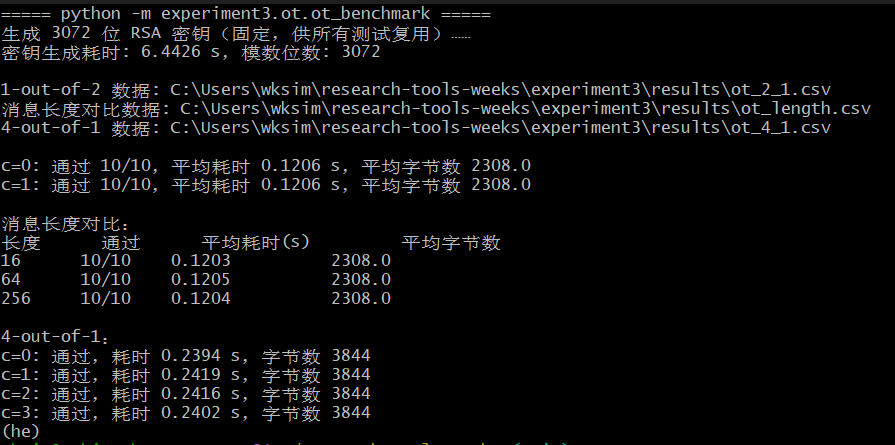
\includegraphics[width=0.92\textwidth]{figures/ot_benchmark.png}
\caption{OT 测试输出（1-out-of-2、消息长度对比与 4-out-of-1 全部通过）}
\label{fig:ot-benchmark}
\end{figure}

\subsection{与直接发送、告知后发送的对比}

\begin{table}[h]
\centering
\caption{三种消息传递方式的隐私对比}
\begin{tabular}{lccc}
\toprule
方式 & S 知道 $c$？ & R 得到几条消息？ & 是否满足 OT 两个隐私目标 \\
\midrule
直接发送两条明文 & 不知道（无选择动作） & 2 条 & 否（R 得到全部） \\
告知 $c$ 后只发所选 & 知道 & 1 条 & 否（S 知道 $c$） \\
RSA 盲化 OT & 不知道 & 1 条（所选） & 是 \\
\bottomrule
\end{tabular}
\end{table}

第一种方式虽然 S 不知道 R“选择了哪条”（因为没有选择动作），但 R 同时拿到两条消息，接收方隐私完全丧失。第二种方式 R 只拿到一条，但 S 直接知道 $c$，发送方隐私完全丧失。OT 同时做到“S 不知道 $c$”和“R 只得到所选消息”，两个目标都满足。

\subsection{消息长度对运行开销的影响}

固定同一对 3072 位 RSA 密钥，只重新生成 $x_0,x_1,k$，分别用 16、64、256 字节的消息各运行 10 次：

\begin{table}[h]
\centering
\caption{不同消息长度下的 OT 开销（固定 RSA 密钥，每组 10 次）}
\begin{tabular}{cccc}
\toprule
消息长度 (字节) & 通过次数 & 平均耗时 (s) & 平均字节数 \\
\midrule
16  & 10/10 & 0.1209 & 2308.0 \\
64  & 10/10 & 0.1208 & 2308.0 \\
256 & 10/10 & 0.1206 & 2308.0 \\
\bottomrule
\end{tabular}
\end{table}

\textbf{分析：}三种长度下\textbf{平均字节数完全相同（2308.0）}，\textbf{耗时也基本持平（约 0.120 s）}。原因是协议把消息嵌入模 $N$ 的整数，线上传输按模数长度固定序列化：S$\to$R 第一轮 $N(384)+e(4)+x_0(384)+x_1(384)=1156$ 字节，R$\to$S 的 $v$ 为 384 字节，S$\to$R 第二轮 $M_0(384)+M_1(384)=768$ 字节，合计 2308 字节。只要 $m_i<N$，消息长度增加不会改变线上字节数；耗时主项是两次模幂，也与消息长度无关。因此\textbf{在 $m<N$ 的范围内，OT 的开销由安全参数决定，不随消息长度变化}。

\subsection{选做：4 选 1 OT}
\label{sec:ot41}

在 1-out-of-2 的基础上直接扩展：S 生成 $x_0,x_1,x_2,x_3$，R 用 $v=(x_c+k^e)\bmod N$ 盲化，S 计算四个 $k_i=(v-x_i)^d\bmod N$ 并发送四个 $M_i$，R 解出 $m_c=(M_c-k)\bmod N$。测试四种选择：

\begin{table}[h]
\centering
\caption{4 选 1 OT 测试结果与 2 选 1 对比}
\begin{tabular}{ccccc}
\toprule
选择位 $c$ & 是否正确 & 耗时 (s) & 字节数 & 对比 \\
\midrule
0 & 通过 & 0.2392 & 3844 & \multirow{4}{*}{约为 2 选 1 的 2 倍} \\
1 & 通过 & 0.2391 & 3844 & \\
2 & 通过 & 0.2397 & 3844 & \\
3 & 通过 & 0.2401 & 3844 & \\
\bottomrule
\end{tabular}
\end{table}

4 选 1 的字节数为 3844，约为 2 选 1（2308）的 1.67 倍；耗时约 0.24 s，约为 2 选 1（0.12 s）的 2 倍。原因是 $x_i$、$k_i$、$M_i$ 的数量从 2 增到 4，S 端的模幂次数从 2 次增到 4 次，耗时随之翻倍；字节数增加主要来自多出的两个 $x_i$ 和两个 $M_i$（各 384 字节），而 $N,e,v$ 保持不变。

% =========================================================
\section{OT 的隐私分析}

\subsection{发送方隐私：S 不知道 R 的选择位}

R 发送给 S 的 $v=(x_c+k^e)\bmod N$ 中，$k$ 是 R 私有、均匀随机的盲化因子。对 S 而言，$k^e\bmod N$ 在 RSA 假设下是伪随机的，$v$ 与 $x_0$、$x_1$ 中的任何一个都没有可区分的关联，因此 S 无法判断 $v$ 对应 $c=0$ 还是 $c=1$。S 收到 $v$ 后只能计算两个 $k_i$，但它不知道哪一个对应 R 的 $k$。

\subsection{接收方隐私：R 只得到所选消息}

R 收到 $M_0,M_1$ 后，只能正确解出 $M_c-k=m_c$。对于 $M_{1-c}$，R 需要 $k_{1-c}=(v-x_{1-c})^d\bmod N$ 才能解出 $m_{1-c}$，但 R 不知道 $d$，也无法从 $M_{1-c}$ 中分离出 $k_{1-c}$。由于 $k_{1-c}\neq k$，用 $M_{1-c}-k$ 得到的是一个与 $m_{1-c}$ 无关的伪随机值。

\subsection{已知条件带来的推断}

若两条消息相同（$m_0=m_1=m$），R 取得其中一条后自然知道另一条也是 $m$，这属于\textbf{已知辅助信息}带来的推断，不是协议额外泄露。若 R 多次运行协议并改变选择，它可以先后取得两条消息，但这与“单次运行中的隐私目标”不同——OT 的隐私目标限定在单次运行内。报告中的测试与实现均按单次运行的语义分析。

% =========================================================
\section{实验总结}

本实验在半诚实模型下完成了百万富翁问题与不经意传输两部分：

\begin{enumerate}
  \item \textbf{基础部分}采用 Paillier 同态加密实现安全比较：Alice 发送 $pk$ 与 $E(a)$，Bob 计算 $E(a-b)$ 并返回，Alice 解密后只判定符号。固定用例 10 条、20 对随机用例全部通过，负数、256、非整数和布尔值都被正确拒绝。三个取值范围（$0\sim15$、$0\sim63$、$0\sim255$）下平均字节数恒为 896.0 字节，协议耗时约 0.0332 s，证明\textbf{开销由安全参数决定，不随输入范围变化}。
  \item \textbf{选做分析}实现二分查询与线性查询：20 个二分样本全部在 8 次内定位 $a$，线性最坏 256 次，二分加速比约 10.8 倍。说明\textbf{单次只泄露 1 比特，但多轮查询的结果组合可推断更具体的财富值}，这是比较函数本身的固有可推断性，防御需限制查询次数或加噪。
  \item \textbf{拓展部分}实现 RSA 盲化 1-out-of-2 OT 与 4 选 1 OT：$c=0$ 和 $c=1$ 各 10 组随机消息全部通过，相同消息和非法选择位也按预期处理；消息长度从 16 增到 256 字节，字节数恒为 2308，耗时约 0.120 s，说明\textbf{OT 的通信与计算开销由 RSA 模数决定，不随消息长度变化}。4 选 1 的字节数为 3844、耗时约 0.24 s，约为 2 选 1 的 2 倍。
\end{enumerate}

通过本实验，我体会到“程序算对结果”不等于“隐私保护有效”：基础比较只暴露 1 比特，但多轮查询仍可推断输入；OT 的两个隐私目标（发送方不知道选择、接收方只得到所选）必须同时由协议结构保证，而不是靠“把两条消息都加密”就能实现。

% =========================================================
\bibliographystyle{plain}
\nocite{*}
\bibliography{reference}

\end{document}